% !TEX TS-program = pdflatex
% !TEX encoding = UTF-8 Unicode

% This is a simple template for a LaTeX document using the "article" class.
% See "book", "report", "letter" for other types of document.

\documentclass[11pt]{article} % use larger type; default would be 10pt

\usepackage[utf8]{inputenc} % set input encoding (not needed with XeLaTeX)

%%% Examples of Article customizations
% These packages are optional, depending whether you want the features they provide.
% See the LaTeX Companion or other references for full information.

%%% PAGE DIMENSIONS
\usepackage{geometry} % to change the page dimensions
\geometry{letterpaper} % or letterpaper (US) or a5paper or....
\geometry{margin=1in} % for example, change the margins to 2 inches all round
% \geometry{landscape} % set up the page for landscape
%   read geometry.pdf for detailed page layout information

\usepackage{graphicx} % support the \includegraphics command and options
\usepackage{hyperref}

\usepackage[parfill]{parskip} % Activate to begin paragraphs with an empty line rather than an indent

%%% PACKAGES
%\usepackage{booktabs} % for much better looking tables
\usepackage{array} % for better arrays (eg matrices) in maths
%\usepackage{paralist} % very flexible & customisable lists (eg. enumerate/itemize, etc.)
\usepackage{verbatim} % adds environment for commenting out blocks of text & for better verbatim
%\usepackage{subfig} % make it possible to include more than one captioned figure/table in a single float
% These packages are all incorporated in the memoir class to one degree or another...

%%% HEADERS & FOOTERS
\usepackage{fancyhdr} % This should be set AFTER setting up the page geometry
\pagestyle{fancy} % options: empty , plain , fancy
\renewcommand{\headrulewidth}{0pt} % customise the layout...
\lhead{}\chead{}\rhead{}
\lfoot{}\cfoot{\thepage}\rfoot{}

%%% END Article customizations


%%% The "real" document content comes below...

\title{Internet Connectivity}
\author{}
\date{} % Activate to display a given date or no date (if empty),
         % otherwise the current date is printed 

\begin{document}
\maketitle

%\begin{quote}
%Wise quote here.\\ \hbox{}\hfil -- {\em A Wise One}
%\end{quote}

\section{Introduction}

With the explosion of computing power and connectivity, the Internet has become a primary means of storing, processing, and delivering data. Cloud computing, social networks, search engines, the ``Internet of Things'' -- each of these require sharing and storage of information, some of it in large quantities (so-called “big data”). This document lays out the fundamentals of using a remote server to store and display information.

The flow of data will happen in several steps, and tutorials and sample code will be provided to help you understand each piece of the puzzle. You’ll start with simple, ``Hello, world!'' applications and work up to a website that displays key statistics of your system (eg, temperatures) and allows you to \emph{control} your greenhouses from the Internet.

\subsection*{Objectives}

Upon successful completion of this lab, the student will be able to:
\begin{itemize}
\item Create a database and multiple, linked tables within it,
\item Implement scripts for retrieving data from a database,
\item Implement scripts for storing data in a database,
\item Transfer data (bi-directionally) between an Arduino and a web server, and
\item Implement a simple web interface for setting control parameters.
\end{itemize}

\subsection*{Preparation}

Before coming to lab, the student should review the following:

\begin{itemize}
\item {\bf Basic LAMP model.} See the overview below as well as Mark Rossi’s notes on collab.
\item {\bf SQL and PHP.} There are links to resources below as well as a good primer by Mark Rossi on collab.
\item {\bf Visit the entire Internet.}
\end{itemize}

Be sure to read through the entire lab before coming to lab.

\section{Overview of information transfer}

The goal over the next few weeks is to connect your greenhouse to the Internet. Doing so will allow you to both monitor and control the greenhouse remotely, key tasks in creating systems in the “Internet of Things”. For this project, the database will live on a virtual machine at Amazon Web Services, and several steps must be accomplished to both store and retrieve information, both from your Arduino and a web browser. Your system will have to connect to the Internet, contact the web server, and send commands to store or retrieve information. You will have to write programs on the server to process incoming requests and build a database to hold all of the data. You’ll need to make a web page to change parameters and visualize information. Each of these steps has its own complications -- there is a lot to do!

Figures~\ref{fig:sending} shows a high level representation of how your system interacts with a database. The steps that are taken include:
\begin{enumerate}
\item The microprocessor (Arduino) that controls your system decides that it needs to send information to or retrieve information from the database,
\item The microprocessor opens a connection to the web server via a WiFi chip and sends a formatted request, which could be either a command to store sensor readings or a request parameters,
\item The server receives the request and invokes the appropriate scripts, which you will write,
\item Those scripts access a database to store/retrieve information,
\item The same scripts send responses back to the web server, which relays the results to your system, and 
\item The microcontroller processes data received through the WiFi chip.
\end{enumerate}

\begin{figure}
\centering
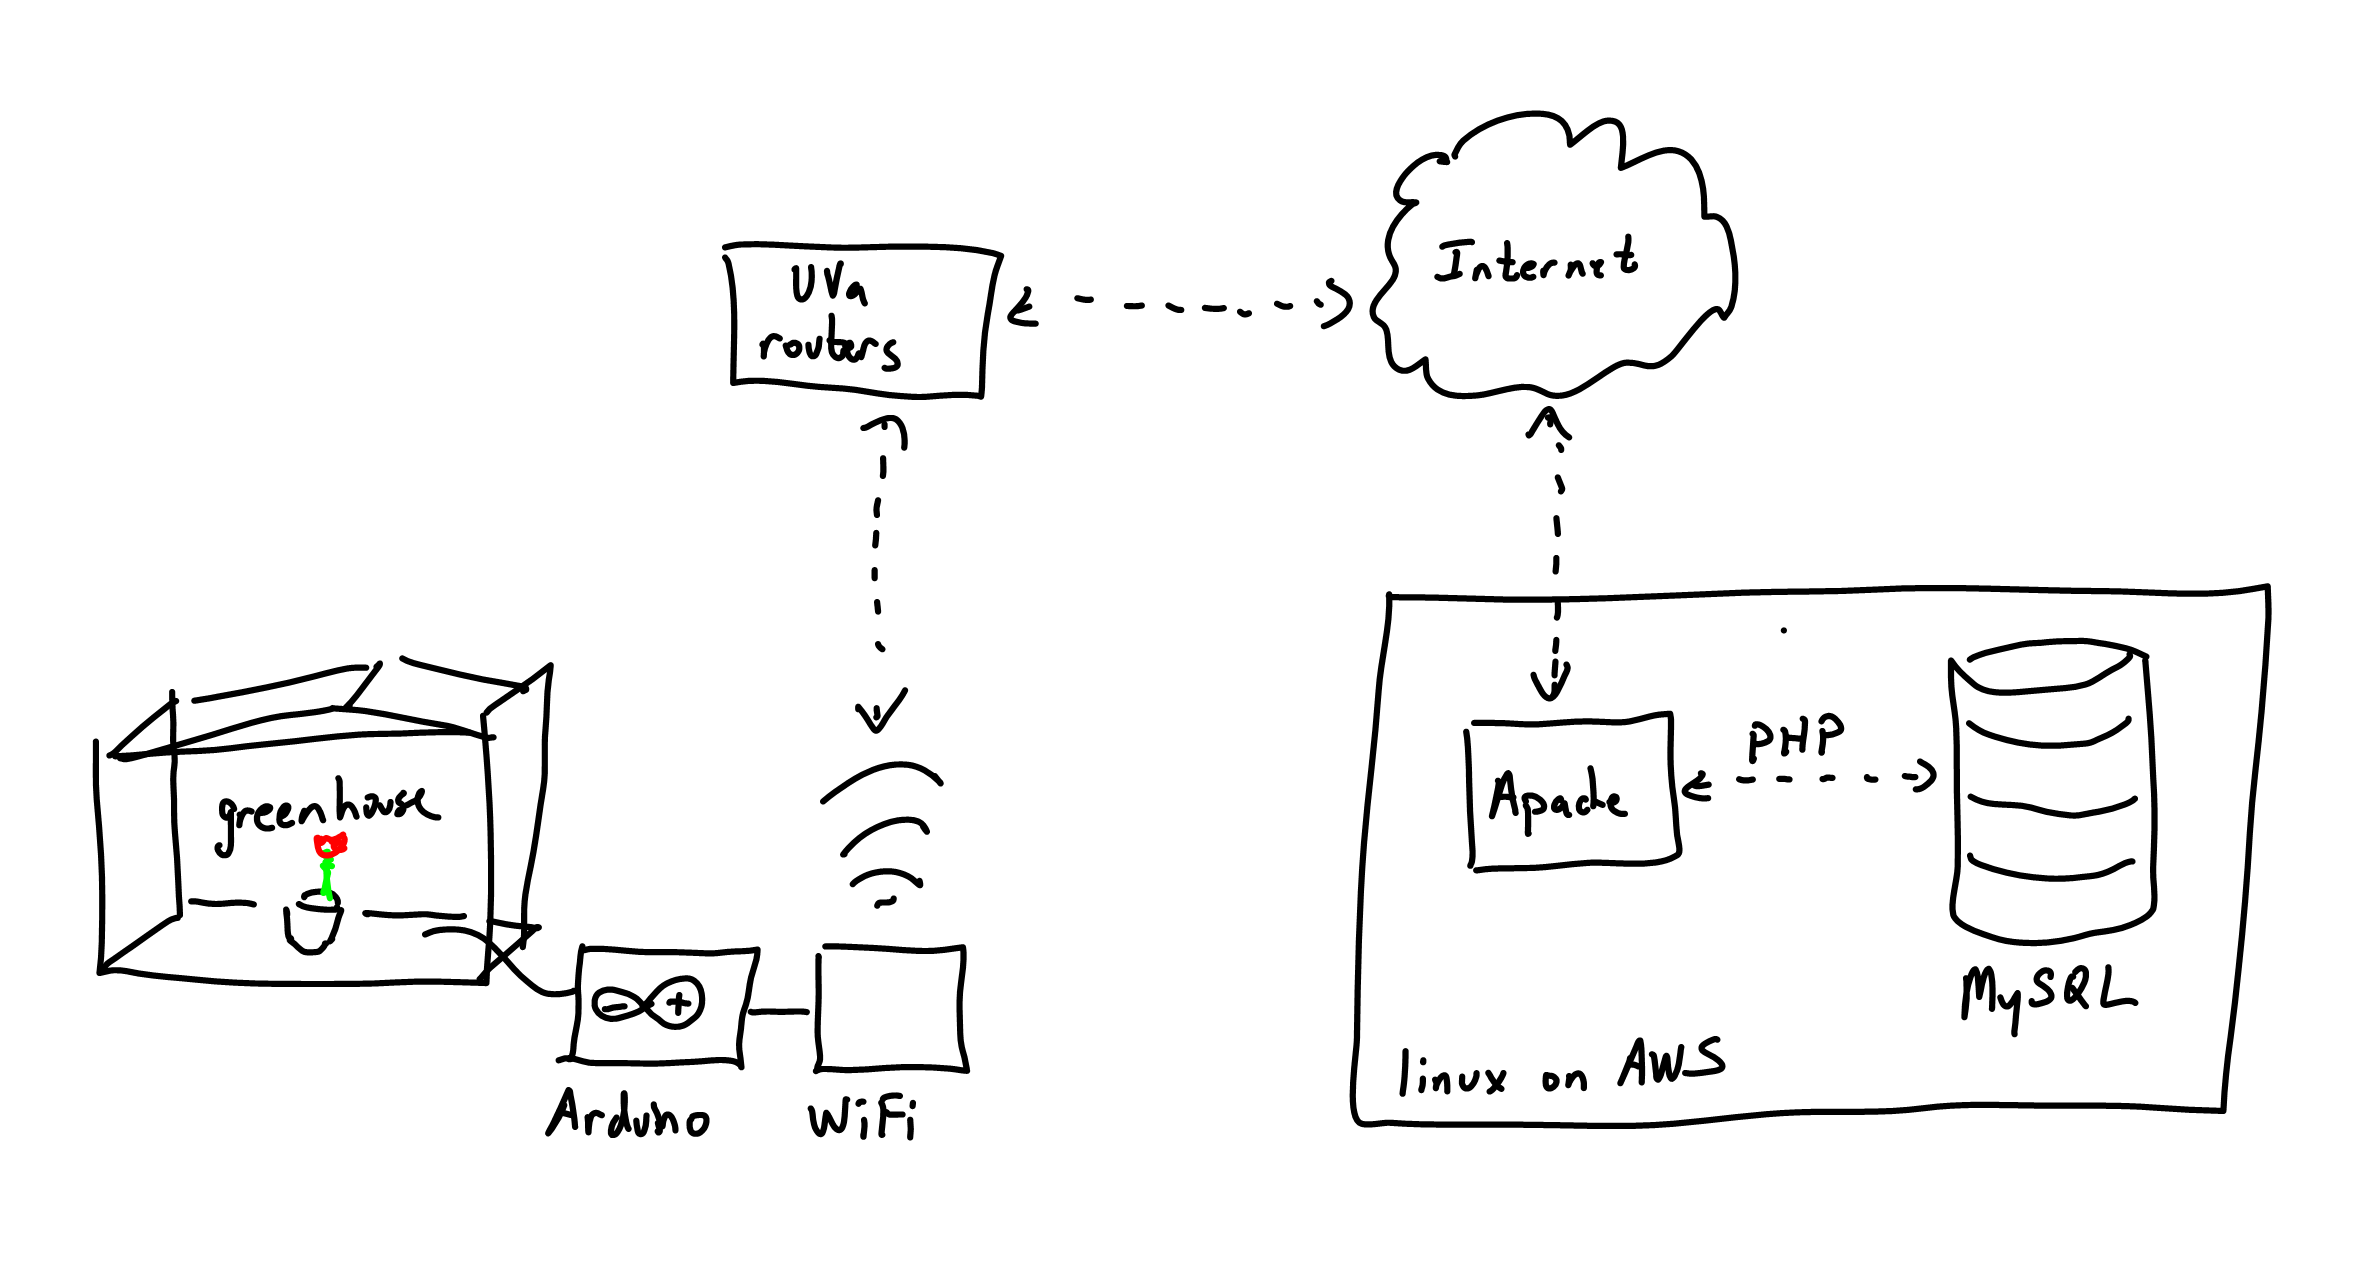
\includegraphics[width=6in]{figures/connections}
\caption{High-level steps needed to send data to a server. See text for description of each step.}% Step 1. Arduino reads data from its sensors, packages it in an http call and sends it to a server. Step 2. On the server, the Apache service receives the request and invokes the desired PHP script. Step 3. The PHP script packages the data into an SQL statement and sends it to a MySQL database.}
\label{fig:sending}
\end{figure}
%
%\begin{figure}
%\centering
%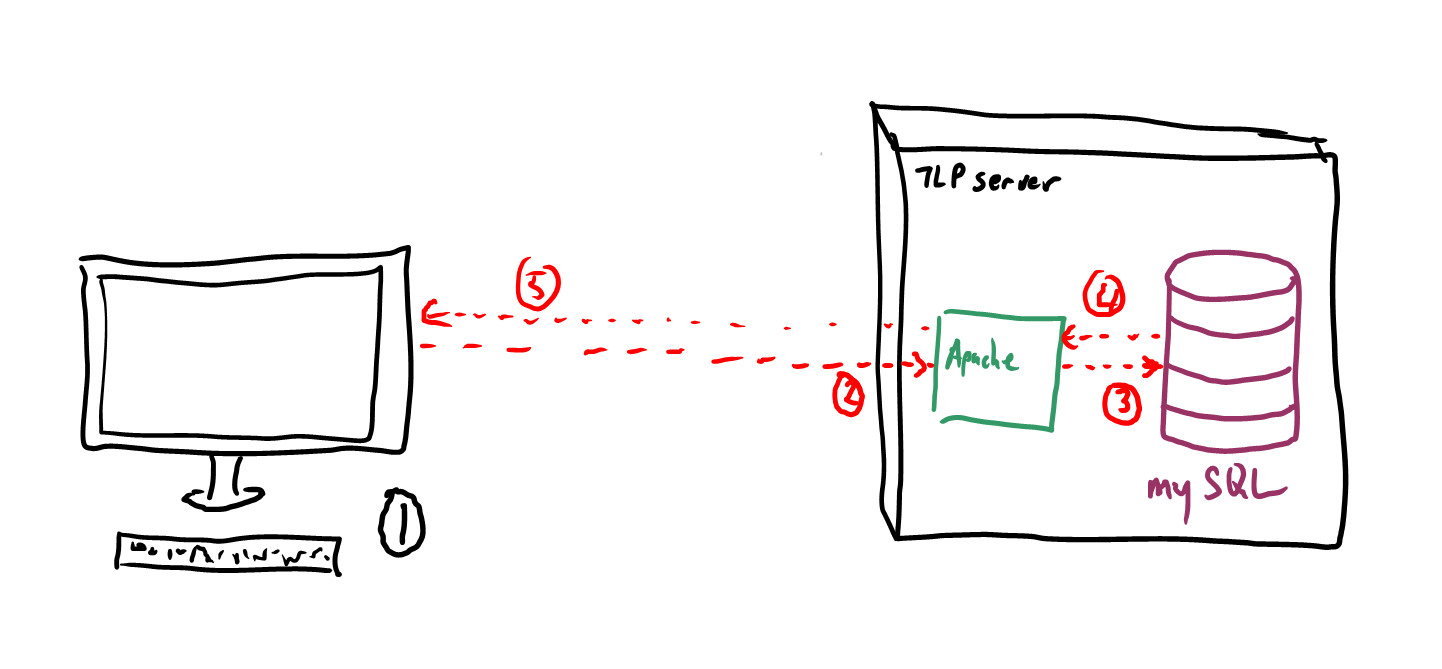
\includegraphics[width=6in ]{figures/retrieving.png}
%\caption{\emph{High-level steps needed to request data from a server.} Step 1. User navigates to a page. The browser makes a request in an http call and sends it to a server. Step 2. On the server, the Apache service receives the request and invokes the requested PHP script. Step 3. The PHP script formats the request as an SQL statement and sends it to a MySQL database. Step 4. The PHP script receives the data from the MySQL database, formats it as either text or as a graphic, and passes it to the Apache service. Step 5. Apache sends the formatted page back to the user.}
%\label{fig:retrieving}
%\end{figure}
%

\subsection*{The LAMP model}

The overview above only lists the high-level steps needed to connect your system to the Internet -- the details for each step are much more complicated and the focus of the rest of this document. On the server side, however, much of the process has been taken care of for you by programs designed specifically to handle these tasks. Specifically, the server is running something called a \emph{LAMP stack}. LAMP is an acronym that stands for Linux, Apache, MySQL, PHP/Perl/Python. {\bf Linux} is the operating system that runs on the server.\footnote{Analogous systems that run Windows are frequently termed WAMP. Mac OS, MAMP.} {\bf Apache} is the program that serves web pages. Basically, it listens for requests on \emph{ports} on the server (eg, \verb|http| requests on port 80) and responds by generating web pages, which may require gathering necessary information for those pages. {\bf MySQL} is a popular database that uses {\bf S}tructured {\bf Q}uery {\bf L}anguage to insert and extract data from the database. {\bf PHP}, {\bf Perl}, and {\bf Python} are all scripting languages that are used to interface with databases (among other things). They are all object-oriented (like Java or C++), but differ in their implementations. This handout focuses on PHP, which is the most common language for scripting web pages, though many of the cool kids are using Python these days. You may use python if you wish, but the examples herein are PHP and your instructor might not be of much help.

Each of the components in the LAMP stack are courses unto themselves. In particular, there are database classes in both Systems Engineering and CS that will give you a deeper understanding of databases and SQL, and there are programming classes where you can learn more about PHP and Python. If you want to get deeper into linux, I’m not going to stop you.

A good reference for SQL can be found at \href{http://www.w3schools.com/sql/default.asp}{\underline{w3schools.com}}. It is unrealistic for you to understand everything on those pages, but you will be responsible for the basics (syntax and the different kinds of statements you can use). {\bf For each of the SQL statements in this lab, be sure to look up the syntax of the statement to see how it works.}

A decent, beginner's tutorial for PHP can be found \href{http://devzone.zend.com/6/php-101-php-for-the-absolute-beginner/}{\underline{here}}, and a quick web search will find many others. There is also a short primer on HTML + PHP for this project written by former student Mark Rossi (’15), found on collab. Again, learning PHP is a course unto itself, but digging into his tutorial to see how things work will help you tremendously.

You will be provided with an account on a virtual linux machine on Amazon Web Services, where you will create a database and PHP scripts. Credentials will be provided separately. As noted, the server is running linux, which has implications for how you can access it:
\begin{itemize}
\item If you're running linux or OSX, you can connect using \verb|ssh|, which stand for “secure shell”. If you're running linux, you presumably know how to do this. If you’re running OSX, you may not be familiar with \verb|ssh|, but help will be provided in class.
\item If you're running Windows 10, my understanding is that it finally has a native \verb|ssh| client -- welcome to the 21st century. It’ll be up to you to figure out how to run it (it’s hidden by default, according to my sources).
\item If you’re running an older version of Windows, or simply want to use a tried and true client, you'll can connect using \verb|putty| or any program that will allow you to login to the server. In the past, students have tried to edit local copies and copy them to the server when needed. Debugging with such a setup is painful. Trust me. 
\end{itemize}

\section{Getting started on the cloud}

Your instructor has set up a virtual LAMP stack on AWS. It’s ‘virtual’ because it is not simply a single computer sitting in a closet. AWS runs an \emph{instance} of a machine on whatever resources it has available. A single machine, or set of machines, at AWS can run multiple instances, all of which appear to be a single machine to us.

Since this is the first year this class has used AWS, there will likely be some unforeseen issues that arise (in particular, access to AWS machines defaults to “very limited”, so your instructor has to specifically open things up for you). As always, your patience is appreciated.

\subsection*{Your account}

Your instructor has what is known as \emph{root privileges} on the server, which means he can create and delete accounts, install useful software like MySQL, adjust security settings, and so forth. With this awesome power, he has created an account for you and set you up with access to MySQL. To log in, you will need an \verb|ssh| client, as noted above.

Logging into your account is not done with a password, but with a public/private key pair. The private key will live on your computer and allow you to login to the machine without having to enter a password. This may sound less secure than a password, but it’s not only more convenient -- it’s also more secure, {\bf so long as the private key remains private!} If someone gets hold of your private key, she or he would have unlimited access to your account, which would be detrimental to your system’s performance, to say the least, and likely have cascading effects on your grade.

Your instructor will provide you with a private key, which you will store on your computer. 

\subsubsection*{Procedure}

\begin{enumerate}
\item Assuming your key is in a file called \verb|fyn.pem|, change to the directory where \verb|fyn.pem| lives, and enter:

\begin{verbatim}
ssh -i "fyn.pem" <comp_id>@ec2-34-209-142-24.us-west-2.compute.amazonaws.com
\end{verbatim}

where \verb|comp_id| is your UVa computing id. You should be immediately logged in to the server, where, you can issue a number of linux commands, including:

\begin{itemize}
\item \verb|ls| will list the files in the current directory. \verb|ls -al| will list all the files (including hidden files) and their permissions.
\item \verb|cd <dir>| changes the current directory to \verb|<dir>|. You can used \verb|cd ..| to go up one directory.
\item \verb|pwd| outputs your present working directory.
\end{itemize}

When you type \verb|ls|, you should see a directory called \verb|public_html|. This directory has been especially set up for serving your particular web files. Any file you put in \verb|public_html| can be found by the \verb|apache| web server and will therefore be publicly available. 

\item To demonstrate, \verb|cd| to the \verb|public_html| directory and type:

\verb|emacs test.txt|

This will open the \verb|emacs| text editor, which is both very powerful and rather archaic. Commands in \verb|emacs| are executed using key combinations, some of which make sense and some of which don’t. If you prefer other text editors (\verb|vi|, \verb|nano|, etc.), feel free to use something else.

\item In your new file, type “hello”. 
\item Type \verb|<ctrl-X> <ctrl-S>| to save and then \verb|<ctrl-X> <ctrl-C>| to close the file. 
\item Point your favorite browser to:

\verb|ec2-34-209-142-24.us-west-2.compute.amazonaws.com/~<comp_id>/test.txt|. 
 
If you see “hello” printed in your browser, congratulations are in order: you’re on the cloud!
\end{enumerate}

\subsection*{PHP scripts}
\label{sec:php.basic}
PHP is a popular language for web scripting, or scripting in general. PHP scripts will provide the connection between the Apache web server and your database. The scripts will be invoked by Apache when a request is made from the Internet, whether from a browser or the Arduino that controls your greenhouse. The scripts will parse the request and interact with your database using SQL commands. Depending on the SQL statements, the script may add information to the database or retrieve data to be displayed. Others may also delete or update records -- it’s all a matter of what you tell the script to do. Before you start to interact with the database, however, you’ll be introduced to the basics of PHP and verify that your account is set up properly.

There are two basic types of PHP scripts: \verb|GET| scripts and \verb|POST| scripts. The fundamental difference is that a \verb|GET| scripts receives information appended to the HTTP request itself, whereas a \verb|POST| script receives information packaged in a separate container. \verb|POST| scripts are more useful when you send lots of data or don’t want to have sensitive information such as passwords printed in clear text in a URL. That said, \verb|GET| scripts are better for learning how the scripts work (and debugging!), so we’ll concentrate on them.

The basic format of a \verb|GET| request is as follows:

\begin{verbatim}
my_script.php?<field1>=<value1>& ... &<fieldN>=<valueN>
\end{verbatim}

where \verb|my_script.php| is the filename of the script and the \verb|?| tells it that a list of \verb|field=value| pairs follows. Each of these pairs will be parsed within the script itself, which allows the user to send search parameters or data to the script.

\subsubsection*{Procedure}

\begin{enumerate}
\item Login to your account on the virtual AWS machine. Switch to your \verb|public_html| directory.
\item Using your favorite editor, open a file called \verb|repeater.php| and add the following to it:

\begin{verbatim}
<?php
$input_str = $_GET[‘input’];
echo $input_str;
?>
\end{verbatim}
\item Save the file and exit the editor.
\item Switch to your favorite browser and enter the following URL (all on one line):

\begin{verbatim}
ec2-34-209-142-24.us-west-2.compute.amazonaws.com/
          ~<comp_id>/repeater.php?input=this is awesome
\end{verbatim}

where \verb|<comp_id>| is your computing ID, of course. Your browser should print “this is awesome” or whatever else you type after the \verb|=| sign.

\end{enumerate}

A few notes:

\begin{itemize}
\item PHP scripts are denoted by the header and footer in the first and last lines of the code above. All PHP code must go between such delimiters, and it is possible to embed PHP within other scripts (e.g., HTML pages).
\item Variables in PHP are denoted by the \verb|$| sign. Note that you don’t need to declare a variable type -- PHP figures out what type of variable to use automatically (which is both a blessing and a curse...).
\item You retrieve the parameters using the format: \verb|$_GET[‘field_name’]|, where \verb|field_name| is the name of the field typed into the URL. In this case, when you entered \verb|input=<some text>|, the script will grab \verb|some_text| and assign it to \verb|$input_str|, which is the variable within the PHP script. Note that \verb|POST| calls work essentially the same, except that they use \verb|$..._POST...$|.
\item A variable can be written to a web page using the \verb|echo| command, which outputs the current value to a stream, which in this case is picked up by the Apache web server for outputting to your browser.
\item Finally, when calling your script from a web browser, you simply prepend the script name with the server name and its location. Apache, running on the server, will then be able to find your script and invoke it. In this case, Apache automatically translates \verb|~<comp_id>| into your \verb|public_html| directory.
\end{itemize}

\section{Creating a database}

A PHP script that simply repeats information isn’t terribly useful, but if you want to interact with a database, you’ll first need to create one. You’ve been given access to MySQL on the server, and full access to a database that shares a name with your computing id (it can be a little confusing that your login id and database name are the same, but MySQL makes it easy to set things up this way).

\subsubsection*{Procedure}

\begin{enumerate}
\item Log in to the AWS virtual machine as you normally do.
\item Enter the database environment by typing: \verb|mysql -u <comp_id> -p|. When prompted for your password, type \verb|tlp_rules|. You may change this if you wish, depending on how well you trust your classmates.
\item The first thing you will need to do is create a database and make it the active one. The only database you have access to will be one with your computing ID, and you will have full permissions on it. At the \verb|mysql| prompt, create a database by typing: \verb|CREATE DATABASE <comp_id>;| Note that the semicolon is necessary, but if you forget it, you can just type it on the next line. Also note that while capitalization does not actually matter, traditional SQL capitalizes keywords -- you may do as you want, but all of the examples here will follow tradition.
\item Type \verb|SHOW DATABASES;|. You will see both your database and another called “information\_schema”, which is a database that contains meta-information about your account.
\item Before you can access a database, you first have to tell MySQL which one you will be using. To do that, type: \verb|use <comp_id>;|
\item You can now list the tables in the database by typing \verb|SHOW TABLES;| Of course, this isn’t particularly interesting, as you have not yet made any.
\end{enumerate}

\subsection*{Creating tables}

A table is the fundamental container for data storage in a database. In MySQL, tables consist of a set of fields, called \emph{columns}, each of which is defined to be a specific data type (e.g., \verb|INT|, \verb|VARCHAR|, a type of string). Records are stored as \emph{rows}, analogous to the rows in a spreadsheet.

There are special attributes that can be assigned to each column to make the database run more efficiently:

\begin{itemize}
\item \verb|PRIMARY KEY|: A primary key is a unique identifier for each record. It helps ensure database integrity, since each record must have a unique primary key. It’s generally good practice to always have a primary key, even if it’s just an \verb|id| field.
\item \verb|INDEX|: When a column is indexed, references to the index are stored in a manner that makes the column much easier to search. For example, if you wanted to find all the records that corresponded to a specific sensor, then indexing \emph{sensor\_id} would allow the database to find the correct records without having to go through the records one by one.
\item \verb|UNIQUE|: Indicates that each row must have a unique value for the specified field. This could be useful for, say, a UVa computing id or your social security number.
\item \verb|NOT NULL|: Indicates that each record must have a value for this field. For a table of sensor readings, it wouldn’t make sense to have empty values for the timestamp, for example. On the other hand, a table of addresses might have an optional field for an apartment number, which would be left empty for many records.
\item \verb|DEFAULT|: The default value that is assigned to a new a record if the value is not otherwise specified.
\item \verb|AUTO INCREMENT|: Similar to default, a way to automatically assign an number that is increased by one with each new record.
\item \verb|FOREIGN KEY|: A way to link two tables together to make data storage more efficient. For example, if an inventory database had a table of orders, it wouldn’t make sense to include the address of the purchaser in each order record. Instead, you could link each order to a customer table, which would store the relevant information in one record.
\end{itemize}

The syntax for each of these options can get confusing, to say the least. If you make mistakes, however, it’s always possible to see the existing table structure using \verb|DESCRIBE TABLE| and make changes using \verb|ALTER TABLE| commands. You can find a complete description of each command in the \href{https://dev.mysql.com/doc/refman/5.7/en/}{\underline{MySQL Manual}}, but that document can be hard to follow so it’s often easiest to just use the search engine of your choice to help you find the correct syntax.

\subsubsection*{Procedure}

\begin{enumerate}
\item If you haven’t already, log in to MySQL and create and select a database with your computing id.
\item Create a table of NCAA basketball teams using the following syntax:

\begin{verbatim}
mysql> CREATE TABLE teams(
   -> team_id INT NOT NULL AUTO_INCREMENT,
   -> university VARCHAR(40) UNIQUE NOT NULL,
   -> mascot VARCHAR(40) NOT NULL,
   -> conference VARCHAR(10),
   -> tournament_region VARCHAR(10),
   -> tournament_seed INT,
   -> PRIMARY KEY ( team_id )
   -> );
\end{verbatim}
\end{enumerate}

Note that you can enter commands on multiple lines -- just enter a semicolon when you’re finished with the complete command.

This table will hold a list of teams and some information about the post season. Note that the primary key is just an index, and \emph{university} has to be unique. The mascot is mandatory (all teams have a mascot), but the conference can be null (for independents) and so can the tournament data, since not every team gets to the NCAA tournament.

Type \verb|DESCRIBE teams| to verify that all the fields are correct.

Now enter some data:

\begin{enumerate}
\item Use the \verb|INSERT| command to add a record:
\begin{verbatim}
mysql> INSERT INTO teams
    -> (university, mascot, conference, tournament_region, tournament_seed)
    -> VALUES
    -> ('UVa', ‘Cavaliers’, ’ACC', 'South', 1);
\end{verbatim}

\item Add a second record
\begin{verbatim}
mysql> INSERT INTO teams
    -> (university, mascot, conference)
    -> VALUES
    -> (‘ISU’, ‘Cyclones’, ‘Big 12’);
\end{verbatim}

\item And a third record
\begin{verbatim}
mysql> INSERT INTO teams
    -> (university, mascot, conference, tournament_region, tournament_seed)
    -> VALUES
    -> (‘Kansas’, ‘Jayhawks’, ‘Big 12’, ‘Midwest’, 1);
\end{verbatim}

\item Now show the records in the table with:

\begin{verbatim}
mysql> SELECT * FROM teams;
\end{verbatim}

You should see three rows. Note that the tournament columns for ISU are \verb|NULL| since the Cyclones didn’t make it to the Big Dance this year (where’s Fred Hoiberg when you need him?).

\item Now select the teams from just the Big 12 conference by qualifying your search with the \verb|WHERE| clause:

\begin{verbatim}
mysql> SELECT * FROM teams WHERE conference = ‘Big 12’;
\end{verbatim}

\item Finally, what do you think will happen if you try entering a fourth record:

\begin{verbatim}
mysql> INSERT INTO teams
    -> (university, conference, tournament_region, tournament_seed)
    -> VALUES
    -> (‘Duke’, ‘ACC’, ‘Midwest’, 2);
\end{verbatim}
\end{enumerate}

You may have expected that the record would be rejected since we declared \emph{mascot} to be \verb|NOT NULL| and we didn’t enter a value. It turns out, however, that there is a difference between a \verb|NULL| value and an empty string. \verb|NULL| means there is no value for a field, whereas an empty string is a value -- it’s just a zero-length string.

\subsection*{Joining tables}
\label{sec:sql.joins}
While it was useful for demonstrating how to make tables, the organization of the database from the preceding section is dismal. An easy way to see this is with a simple demonstration.

\subsubsection*{Procedure}

\begin{enumerate}
\item Add another record, being careful to enter the conference verbatim:

\begin{verbatim}
mysql> INSERT INTO teams
    -> (university, mascot, conference)
    -> VALUES
    -> (‘KSU’, ‘Wildcats’, ‘Big12’);
\end{verbatim}

\item Re-enter (or use the up arrow to scroll though your history) the \verb|SELECT ... WHERE| statement above. What do you see?

\end{enumerate}

The problem is that there is no way of ensuring that the names of the conferences are consistent. You could enter, “Big 12”, “Big12”, “Big Twelve”, or even “Big 0x0C” and the database would blindly accept them all. \underline{A fundamental “best practice” of relational databases is to avoid repeated data}, and the best way to do that is to divide data up into multiple tables, each of which holds a minimal dataset. Let’s work through an example.

\subsubsection*{Procedure}

\begin{enumerate}
\item Create another table, called \emph{conferences}, with the following structure:
\begin{itemize}
\item \emph{conference\_id} as the \verb|primary key| with \verb|AUTO_INCREMENT|, and
\item a \verb|NOT NULL| \emph{conference\_name}.
\end{itemize}
\item Use \verb|INSERT INTO| to add entries for the Big 12 and the ACC.
\item Alter the \emph{teams} table as follows:
\begin{verbatim}
mysql> ALTER TABLE teams DROP conference;
mysql> ALTER TABLE teams ADD conference_id INT DEFAULT NULL;
\end{verbatim}
\item Now assign teams to a conference using the \verb|UPDATE| statement:
\begin{verbatim}
mysql> UPDATE teams SET conference_id = 1 WHERE university = ‘ISU’;
\end{verbatim}
Do this for each entry in the \emph{teams} table.
\item Now enter the following:

\begin{verbatim}
mysql> SELECT university, conference_name FROM teams
     -> INNER JOIN conferences ON
     -> teams.conference_id=conferences.conference_id;
\end{verbatim}
\end{enumerate}

You should see a list universities and their conferences. The form of the statement is a little hard to remember, but it’s easy enough to do a web search to get the syntax correct. The important point is that we define an \verb|INNER JOIN| to create what looks like a new (but temporary) table with information from multiple sources. \emph{The power of relational databases is that it is possible to combine information from multiple tables to meet the specific needs of the user.}

\subsection*{Foreign keys}

Let’s break the database once again.

\subsubsection*{Procedure}

\begin{enumerate}
\item Add another team:

\begin{verbatim}
mysql> INSERT INTO teams
    -> (university, mascot, conference)
    -> VALUES
    -> (‘Carleton College’, ‘Golden Knights’, 3);
\end{verbatim}

\item Execute the previous \verb|JOIN| query. Where is Carleton?
\end{enumerate}

The problem now is that there is nothing that ensure that the specific conference id exists in the converences table. What we really want is to ensure that the conference field is correct, and we can do this with something called \emph{foreign keys}. Foreign keys are formal links between tables within a database that can be used to guarantee data integrity. Before you add one though, you’ll need to put in a proper entry (and get some more practice!):

\subsubsection*{Procedure}

\begin{enumerate}
\item Add a conference record for the MIAC conference. Use a \verb|SELECT| statement to determine its \emph{conference\_id}. Make sure it matches the \emph{conference\_id} for Carleton College in \emph{teams}.
\item Add a foreign key to the \emph{conference\_id} as follows:

\begin{verbatim}
mysql> ALTER TABLE teams
    -> ADD FOREIGN KEY fk_conf(conference_id)
    -> REFERENCES conferences(conference_id)
    -> ON DELETE CASCADE
    -> ON UPDATE CASCADE;
\end{verbatim}

\item Repeat the university/conference query from before. Is Carleton there now?
\item Now try adding a university in an entirely new conference. What happens?
\end{enumerate}

\section{Web interface}

Now that you’ve seen how to create and manipulate databases, it’s time to write more powerful PHP scripts that can interact dynamically with the data in your database. The basic premise is straightforward: we’ll have PHP scripts perform SQL statements and pipe the results to a web page. We’ll get started once again with an example.

\subsubsection*{Procedure}

\begin{enumerate}
\item Type ‘quit’ to exit the MySQL environment. On your local machine, grab a copy of \verb|teams.php| from collab and upload it to the server with \verb|scp|, which is short for “secure copy”. Type the following all on one line:
\begin{verbatim}
scp -i "fyn.pem" teams.php <comp_id>
@ec2-34-209-142-24.us-west-2.compute.amazonaws.com:public_html
\end{verbatim}
\item On the AWS server, \verb|cd| to the \verb|public_html| directory and open the file in \verb|emacs| or your favorite editor.
\item Change the lines starting with \verb|$db_user| and \verb|$db_pass| to reflect your username and MySQL password. Set \verb|$database| to your computing id (which is also the name of your database). Save the file.
\item Point your favorite web browser to:
 
\verb|ec2-34-209-142-24.us-west-2.compute.amazonaws.com/~<comp_id>/teams.php|

If all goes well, you should see the result of the query you did in Section~\ref{sec:sql.joins}.
\end{enumerate}

The ability to query the database from a web browser if useful, but the real power lies in being able to query on specific criteria. Using the code from Section~\ref{sec:php.basic} as a guide, edit your PHP script to accept \emph{conference\_name} as an input. Then alter the SQL statement so that it only returns teams in the specified conference. To so this, you’ll need to make use of the \verb|WHERE| clause:

\begin{verbatim}
"...WHERE conference_name = '$conf_name’...”;
\end{verbatim}

where I’ve assumed a variable named \verb|$conf_name|. Note that the entire query must be in double quotes and the variable in single quotes. This tells PHP to interpret the variable as its actual value and then the query literally.

\clearpage
\section*{Assignment (5 points)}

{\bf This is an individual assignment. Due Wednesday, 3/28 at the start of class.} 

\begin{enumerate}
\item {\bf Create a table to hold sensors.} Create a table called ``sensors'' with four fields:
\begin{itemize}
\item \emph{id} of type \verb|INT|,
\item \emph{name} of type \verb|VARCHAR(32)|,
\item \emph{short\_name} of type \verb|VARCHAR(12) UNIQUE|, and
\item \emph{units} of type \verb|VARCHAR(12)|.
\end{itemize}
Set \emph{id} as the \verb|PRIMARY KEY|. Make all of the fields \verb|NOT NULL|.
\item {\bf Create a table to hold readings.} Create a table called ``sensor\_readings''. Add the following fields:
\begin{itemize}
\item \emph{id} of type \verb|INT AUTO_INCREMENT|,
\item \emph{sensor\_id} of type \verb|INT|,
\item \emph{time\_stamp} of type \verb|TIMESTAMP|, defaulted to \verb|CURRENT_TIMESTAMP|, and
\item \emph{value} of type \verb|DECIMAL (5,2)|. Make the \emph{id} field a \verb|PRIMARY KEY|. Make the \emph{sensor\_id} field indexed using \verb| KEY `sensor_sid` (`sensor_id`)|. Make all of the fields \verb|NOT NULL|.
\item Create a link (foreign key) from \emph{sensor\_readings.sensor\_id} to \emph{sensors.id}.
\end{itemize}
\item {\bf Insert some data.} 
\begin{itemize}
\item Insert two sensors: 
\begin{enumerate}
\item Inside temperature: Set \emph{id} to \verb|1| and \emph{short\_name} to \verb|T_in|. We roll Celsius in this class.
\item Outside temperature: Set \emph{id} to \verb|2| and \emph{short\_name} to \verb|T_out|.
\end{enumerate}
\item Insert several readings for each sensor. Note that the \emph{time\_stamp} should default to the current time on the server, so you'll need to remove references to it in your \verb|INSERT| statement.
\end{itemize}
\item {\bf Make it interactive.}
\begin{itemize}
\item Write an SQL statement to SELECT all of the readings of sensor 1. Write the SQL statement here:
\vspace{0.25in}
\item Following the format for joining tables, write a statement to select all of the readings the sensor with the \emph{short\_name} of \verb|T_out|. Write out the result as: \emph{name, timestamp, value, units}. Write the SQL statement here:
\vspace{0.25in}
\item Write a PHP script that accepts \emph{short\_name} as a parameter and returns the results of the previous query. Write out the result as: \emph{name, timestamp, value, units}. Write the URL here:
\end{itemize}
\end{enumerate}
\end{document}
\clearpage
\section{Communication from a microcontroller}

In addition to the hardware already provided, each group will be provided the following:
\begin{itemize}
\item A \href{https://www.adafruit.com/products/1469}{\underline{CC3000 WiFi breakout board}} from Adafruit. In the interest of full disclosure, this is the first time the class will use the CC3000 -- in previous editions, students used the Arduino Ethernet shield, which resulted in cables strung all over the lab. Your professor has successfully tested the CC3000 with the wahoo network, but that’s no guarantee that things will go perfectly smoothly!
\end{itemize}

The CC3000 uses SPI to communicate with your Arduino. Remember how SPI works? Good, because it will likely show up on a quiz.

\subsection{Basic connectivity}
The first thing to do is make sure that you can connect your Arduino to the Internet. Working with your team, you’ll demonstrate that you can make a network connection and read a trivial webpage with your Arduino + CC3000 WiFi. {\bf If you have trouble with any of the tutorials, see an instructor sooner rather than later.} Again, all of these tutorials have been tested, but unforeseen issues may arise.
\begin{enumerate}
\item Go to the Adafruit page for the CC3000 and work through the tutorials up to and including WebClient. If you have not yet soldered pins onto your breakout board yet, now is your chance. You will be connecting to the unsecured \verb|wahoo| network using the following parameters:
\begin{verbatim}
#define WLAN_SSID       "wahoo"     
#define WLAN_PASS       ""
#define WLAN_SECURITY   WLAN_SEC_UNSEC
\end{verbatim}
\end{enumerate}

Note that the tutorial sketches make copious use of two macros, \verb|fastrprint()| and \verb|F()|.
\begin{itemize}
\item \verb|fastrprint()| is a special library for printing that doesn’t use as much of the Arduino’s resources. Basically, \verb|fastrprint()| allows the Arduino to send an http request as one packet, as opposed to individual packets for each character. Note that \verb|fastrprint()| is limited to 90 characters per string -- be careful not to exceed that limit.
\item The \verb|F()| macro tells the Arduino to store string literals in the program code (flash memory) instead of the default RAM. The Atmega328 is limited to 2kB RAM, but it has room for 32kB of program code. For code that is heavy in strings (as are many sketches for connecting to the Internet), it is useful to put the strings in program memory.
\end{itemize}

\subsection{Sending data to a database}
\label{sec:who.are.you}
Once you’ve demonstrated basic connectivity, the next step is to send information to a database. You’ll do this by invoking an CC3000 Client object and ``printing'' html commands to it, much the same way as you print to the Serial Monitor or an SD card. In this case, however, you’ll ask the server to invoke a PHP script, which will insert data into a database. The PHP script will use the GET protocol to parse the data. With the GET prototcol, the data are included in the http request string (essentially, the URL) with the following format:
\begin{verbatim}
  http://<hostname>/<scriptname>?<variable1>=<value1>&<variable2>=<value2>...
\end{verbatim}
The \verb|?| character tells the script that a list of \verb|variable=value| pairs is coming, each separated by the \verb|&| character. An alternative method is to package data first and send it using the POST protocol. This is most often done with large datasets, such as from a web form, or when you need to conceal a password.

\begin{enumerate}
\item Find the section of the WebClient sketch where it requests the webpage. Rewrite the code so that it connects to \verb|128.143.6.188/tlp/gcl8a/addtoroster.php|\footnote{A copy of the PHP script has been put on collab for reference, though you don’t need to do anything with it.} and sends the following as part of the \verb|GET| statement:
\begin{itemize}
\item id = [your computing id]
\item firstName = [your first name]
\item lastName = [your last name]
\item year = [your year of graduation]
\item favoritePizza = [your favorite pizza]
\end{itemize}

You’ll need to set the ip address to \verb|128.143.6.188|. 

You will also need to replace the line \verb|www.fastrprint(WEBPAGE)| with the name of the PHP script and add additional lines to report each piece of data using the \verb|GET| format above. Be sure to leave the request in the \verb|setup()| section of your sketch, so it is only called once. Upload the sketch to your Arduino and run it.
\item When complete, point a browser to \href{http://128.143.6.188/tlp/gcl8a/getroster.php}{\underline{http://128.143.6.188/tlp/gcl8a/getroster.php}} and check if your name is there. If it is, well done. If not, find an instructor.
\item Repeat the above for each member of your team.
\end{enumerate}

{\bf Show an instructor that you have entered the data.}

\vspace{0.25in}
Instructor initials: \rule{2in}{0.4pt}
\vspace{0.25in}

\subsection{Debugging PHP scripts}

Debugging PHP scripts is a pain. It’s very easy to make syntax errors -- especially with quotation marks -- and the scripts often don’t fail nicely. For example, you may put a debug \verb|echo| statement early in the script, hoping that will prove your script made it that far, but even if the error is after the \verb|echo|, it usually won’t print. One way to find the offending statement is to comment out the majority of the script and add the statements back line-by-line until you find which statement is causing the problem. If you \verb|ssh| to the server directly (easily done on a Mac; it requires additional software on a Windows machine), things will go much faster because you can edit the script directly instead of re-uploading the file each time you make a change.

One problem that we see frequently is that students don’t know if the problem is in their script or their Arduino sketch. It is quite easy to test a PHP script directly just by using a web browser. Simply point your browser to the script and manually enter all of the fields -- that’s all your Arduino is doing, anyway.

As an example, your professor has made a trivial database for “screaming into the void”. Replacing the placeholders appropriately, point your browser to
\begin{verbatim}
128.143.6.188/tlp/gcl8a/screamintothevoid.php?name=<your name>&scream=<your scream>
\end{verbatim}

where the fields are in the standard format described above. Note that your scream can’t have any apostrophes or quotes in it.

To see your and your classmates’ frustrations, point your browser to
\begin{verbatim}
128.143.6.188/tlp/gcl8a/peerintothevoid.php
\end{verbatim}

Whenever you have troubles writing to a database, in general, you should first confirm that you have a working PHP script using steps similar to that above before you start worrying about your Arduino sketch.

\subsection{Storing greenhouse data in a database}

Now that you understand how to invoke PHP scripts from your Arduino, it’s time to start writing temperature (and other) data to a database. To do this, you will have to combine elements of your existing greenhouse code (the one that writes to an SD card every 10 seconds) and the WebClient code from above. Using the database you created as part of the Pre-lab (in Section~\ref{sec:pre.lab} -- don't forget to do the prelab), write a sketch that will periodically poll the temperature sensors and send the values to your database. Specifically,

\begin{enumerate}
\item Download a copy of \verb|addtoroster.php| from collab. This script shows the basic format for using GET to receive and parse data into a database.
\item Edit the script to process your sensor readings. You will have to edit/add lines to parse the GET fields as well as change the SQL statement and database. Also, you will need to add the user id and password for your \verb|phpmyAdmin| account near the top. \emph{Important note}: Because you set the timestamp field in your database to default to the current time, you shouldn't specify anything for that field -- MySQL will take care of it for you. Place the script in the \verb|web/| directory under your home directory. Test your script using a web browser -- you can check if the data made it using \verb|phpmyAdmin|.

Note that the URL for your scripts will be \verb|/tlp2018/<user id>/<script>.php|.
\item Combine your most recent Arduino greenhouse sketch with the WebClient sketch so that, instead of storing data to the SD card, you send the interior temperature, the exterior temperature, the set-point, and the power generated at the heater (in Watts, not just ON/OFF) to your database.
\item Print the readings to the Serial Monitor so you can verify that the data is correct.
\item Upload the sketch and open the Serial Monitor. Let the sketch run for a minute or two.
\item In \verb|phpmyadmin|, click on your data table and click ``Browse''. You should see several lines of data -- verify that the data is correct as well as the timestamp. If you don’t, see an instructor.
\end{enumerate}

{\bf Show your working system to an instructor.}

\vspace{0.25in}
Instructor initials: \rule{2in}{0.4pt}
\vspace{0.25in}

\subsection{Retrieving information from the database}

The last thing we'll do is get data \emph{from} your database and use it in your Arduino sketch. Specifically, you'll make a web page that allows you to control the set-point of your greenhouse remotely. First, let's verify that your Arduino can receive information:

\begin{enumerate}
\item Edit the WebClient sketch to invoke a PHP script at \verb|128.143.6.188/greg/get_current.php|, a copy of which is found on collab. You can also make a copy if you’re on the server by moving to your \verb|web/| directory and typing 

\verb|cp /var/www/tlp/greg/greenhouse/get_current.php .|

This script retrieves the last row of data from the temperature database for my house and echoes it to a web page. (It's not formatted to be pretty, but it has the format: timestamp; indoor temp., outdoor temp.
\item Upload your new sketch and open the Serial Monitor. If all went well, you should see the current indoor and outdoor temperatures at my house (along with a mess of html tags and other data).

If not, see an instructor.
\end{enumerate}

Once that works, you'll need to make a webpage that accepts user input and stores the value to a database that your Arduino can access. A copy of \verb|changesetpoint.html| has been put on collab. A similar file in your professor's directory on the TLP server creates the web page that can be seen at \verb|http://128.143.6.188/tlp/greg/greenhouse/changesetpoint|. This page allows the user to enter a desired set-point, does a \emph{very basic} security check, and puts the set-point in a database. You can get a copy by moving to your \verb|web/| directory and typing 

\verb|cp /var/www/tlp/greg/greenhouse/get_current.php .| 

You'll need to:
\begin{enumerate}
\item Create a table that holds the desired set-point. This is different from the recorded set-point in the table you made above. Be sure to add an id field and a timestamp to keep track of when the set-point was updated.
\item Edit the provided web page code so that it points to your new table, and adjust the permissions as needed. Save it in your \verb|web/| directory.
\item Create a PHP script that returns the current set-point, ie, the most recent record.% This script should return the set-point if the time is between 6:00 AM and 8:00 PM; otherwise, it should return the set-point minus the set-back. Look at Figure~\ref{fig:???} to see how to do time comparisons.
\item Using the WebClient sketch as a template, periodically poll the server, parse the return string, and print the set-point to the Serial Monitor. Note that your PHP script will return much more than the set-point itself; it will be useful to enclose the set-point in a tag, eg. \verb|<setpoint>25</setpoint>|. Then you can search each line using the \verb|startsWith()| and \verb|endsWith()| methods.
\end{enumerate}

If all goes well, you should be able to change the set-point from a standard web browser and see the changes printed in the Serial Monitor.

\section{Putting it all together}

Let's see...you now have an Arduino that monitors and controls the temperature in your greenhouse, and the infrastructure to view and change parameters from a web browser (at the moment, stored data can only be accessed in text form -- we'll add graphics later). It's time to put it all together. Your task is to build a system with the following functionality:

\begin{itemize}
\item As before, temperature control with a 1C hysteresis band.
\item A heating set-point (with set-back) that can be controlled from the Internet. Note that you should remove the buttons that were previously used for changing the set-point.% Set-back will be controlled by the time: if the current time is between 10pm and 6am, the system will drop the set-point by 2C. There is a PHP function called \verb|localtime()| to get the current time.
\item A cooling set-point such that when it gets too hot, the lid will open. You should already have this.% The cooling set-point must also be controlled from the Internet. The cooling set-point does not need a set-back period.
\item Stores interior and exterior temperatures, current set-point, and power to the heater in a database on the TLP server. Also, add a flag for the position of the lid. Write the data every 30 seconds.
\item Continue to write temperature and set-point data to the LCD, as before.
\end{itemize}

\end{document}

\section{Making fancy displays}

{\bf To be discussed in class on Thursday, 3/31.}

The final step in connecting your greenhouses to the internet is to make the data accessible to all of your fans (trust me, this is important!). In this case we'll create a web page that graphs the data using Highcharts, a popular graphing package written in javascript. An example chart, made by your professor to view the temperature data at his house, can be found at \verb|http://128.143.6.188/greg/display_mysql.php?days=2|, which shows the indoor and outdoor temperatures for the last 2 days. It also shows supply and return temperatures and the state of the fan if you click on the appropriate spot in the legend.

The file for creating the page above, with copious annotations, has been put on collab. Your task is to put a copy of this file in your \verb|web| directory and edit it to display data gathered from your greenhouse. You are encouraged to change some of the options to ``customize'' your page, and you can visit \verb|www.highcharts.com| to see all of the crazy things you can do with Highcharts. Bar charts, column charts, line charts, stock charts, pie charts, most any kind of chart is pretty straighforward, so have fun with it!

\clearpage
\section{Pre-lab}
\label{sec:pre.lab}

{\bf This is an individual assignment. Due at the beginning of lab.} (See what you are delivering at the bottom of the assignment.)

Each of you have been given an account and a database on the ``TLP Server'', a linux machine physically living in my office and virtually living at \verb|128.143.6.188|. Your login credentials will be given separately. Note that logging in to the machine (your account) is different than logging into the database manager (\verb|phpmyAdmin|). With the latter, you can't do much more than manage your database, but this is the only practical way to do so. When uploading PHP or HTML files, you’ll put them in a \verb|web| subdirectory under your home directory, which is linked to the web server folders. Thus, when uploaded scripts, you only need to store them in \verb|128.143.6.188/<your name>/web/| and they will be accessible to the web server.

\begin{enumerate}
\item {\bf Create a database.} Login to phpmyadmin by navigating to \verb|128.143.6.188\phpmyadmin| and entering your credentials. You should already have a database with the same name as your email id. If not, click on ``Databases'' and create a new one with the same name as your email id.
\item {\bf Create a table.} Create a table called ``sensors''. Add three fields:
\begin{itemize}
\item \emph{id} of type integer, AUTO\_INCREMENT, PRIMARY KEY,
\item \emph{name} of type var\_char(32),
\item \emph{display\_name} of type var\_char(32), and
\item \emph{units} of type var\_char(32).
\end{itemize}
\item {\bf Create a second table.} Create a table called ``sensor\_readings''. Add the following fields:
\begin{itemize}
\item \emph{id} of type integer, indexed
\item \emph{time\_stamp} of type timestamp, default to CURRENT\_TIMESTAMP, and
\item \emph{value} of type float.
\end{itemize}
\item {\bf Insert some data.} 
\begin{itemize}
\item Click on ``SQL''. Here you can perform most any SQL statement, and it has convenient templates for performing common operations.\footnote{You have to be careful, though, the default DELETE statement -- if you execute it -- will delete everything in the selected table permanently, and without much warning.}
\item INSERT two sensors: an inside temperature and an outside temperature. Note that the id should default to AUTO\_INCREMENT, so you'll need to remove references to it in your INSERT statement. You’ll use “display\_name” for your graph later, so make it reasonably descriptive. Click on ``Browse'' to make sure the records were inserted properly. For now, just keep track of which sensor has which id.
\item INSERT a few readings for each sensor. Note that the time\_stamp should default to the current time on the server, so you'll need to remove references to it in your INSERT statement.
\item SELECT all of the readings of sensor 1.
\item Following the format for JOINing tables (in Mark's handout), SELECT all of the readings of sensor 1, such that the results also show the display\_name field.
\end{itemize}
\end{enumerate}

Save this last SQL statement! You’ll show it to an instructor upon arrival in lab, which will demonstrate that you have done the prelab and you can write a basic SQL statement.

\vspace{0.25in}
Instructor initials: \rule{2in}{0.4pt}
\vspace{0.25in}

\end{document}

